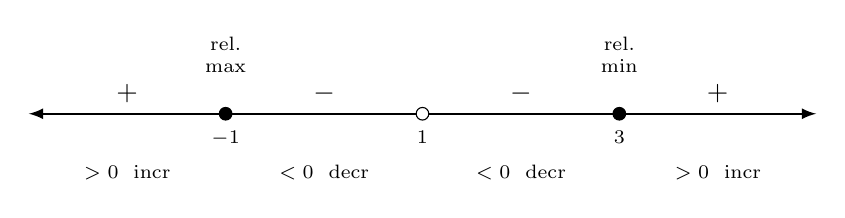
\begin{tikzpicture}[>=latex]

\draw [<->, thick] (-5,0) -- (5,0);
\foreach \x / \y  in %
					{%
					-2.5/{$-1$},%
					2.5/{$3$}%
					}
		{\draw [fill] (\x,0) circle [radius=0.08];
		 \draw (\x,-0.1) node[below] {\scriptsize \parbox{40pt}{\centering \y}};}
\draw [fill=white] (0,0) circle [radius=0.08];
\draw (0,-0.1) node[below] {\scriptsize \parbox{40pt}{\centering $1$}};
\draw (-3.75,-.75) node {\scriptsize \parbox{50pt}{\centering $\fp>0$ \ incr }};
\draw (-3.75,.25) node {$+$};
\draw (-1.25,-.75) node {\scriptsize \parbox{50pt}{\centering $\fp<0$ \ decr }};
\draw (-1.25,.25) node {$-$};
\draw (1.25,-.75) node {\scriptsize \parbox{50pt}{\centering $\fp<0$ \ decr }};
\draw (1.25,.25) node {$-$};
\draw (3.75,-.75) node {\scriptsize \parbox{50pt}{\centering $\fp>0$ \ incr}};
\draw (3.75,.25) node {$+$};
\draw (-2.5,.75) node {\scriptsize\parbox{15pt}{\centering rel. max}};
\draw (2.5,.75) node {\scriptsize\parbox{15pt}{\centering rel. min}};
\end{tikzpicture}
